\begin{abstract}

  \textbf{1. }
    Phylogenetic trees are currently routinely reconstructed from an alignment 
    of character sequences (usually nucleotide sequences). 
    Bayesian tools, such as MrBayes, RevBayes and BEAST2, 
    have gained much popularity over the last decade, 
    as they allow joint estimation of the posterior distribution of the 
    phylogenetic trees and the parameters of the underlying inference model.  
    An important ingredient of these Bayesian approaches is the species tree 
    prior.
    In principle, the Bayesian framework allows for comparing 
    different tree priors, which may elucidate the macroevolutionary 
    processes underlying the species tree.
    In practice, however, only macroevolutionary models that allow for fast computation of the prior probability are used.
    The question is how accurate the tree estimation is when the real macroevolutionary processes are substantially different from those assumed in the tree prior. \\
    \textbf{2. }
    Here we present \verb;pirouette;, 
    a free and open-source R package that assesses 
    the inference error made by Bayesian phylogenetics for a given macroevolutionary diversification model. \verb;pirouette; makes use of 
    BEAST2, but its philosophy applies to any Bayesian phylogenetic inference 
    tool. \\
  \textbf{3. }
    We describe \verb;pirouette;'s usage \new{providing full examples in which 
    we interrogate a model for its power to describe another.
    \\
  \textbf{4. }
    Last, we discuss the results obtained by the examples and their 
    interpretation. \\
\end{abstract}

{\bf Keywords:} Bayesian model selection, BEAST2, computational biology, evolution, phylogenetics, R, tree prior

%%%%%%%%%%%%%%%%%%%%%%%%%%%%%%%%%%%%%%%%%%%%%%%%%%%%%%%%%%%%%%%%%%%%%%%%%%%%%%%%
\section{Introduction}
%%%%%%%%%%%%%%%%%%%%%%%%%%%%%%%%%%%%%%%%%%%%%%%%%%%%%%%%%%%%%%%%%%%%%%%%%%%%%%%%

The development of new powerful Bayesian phylogenetic inference tools, 
such as BEAST [\cite{drummond2007beast}], 
MrBayes [\cite{huelsenbeck2001mrbayes}]
or RevBayes [\cite{hohna2016revbayes}] 
has been a major advance in constructing phylogenetic trees 
from character data (usually nucleotide sequences) extracted
% 00004
from organisms (usually extant, but extinction events 
and/or time-stamped data can be added), 
and hence in our understanding of the main drivers 
and modes of diversification \richel{Reword this awkwardly long sentence}.


BEAST [\cite{drummond2007beast}] is a typical Bayesian phylogenetics tool, 
that needs both character data and priors to infer 
a posterior distribution of phylogenies.
Specifically, for the species tree prior - which describes 
the process of diversification - 
BEAST has built-in priors such as the Yule [\cite{yule}] and 
(constant-rate) birth-death [\cite{nee1994reconstructed}] models.
These simple tree priors are \new{among} the most commonly used, 
as they represent some biologically realistic processes (i.e. 
branching at per species constant rates), while being computationally fast.

\new{
  % 00002
  In this paper, we focus on BD models, instead of coalescent models,
  although these are just as important. Coalescent models ... 
  [RJCB: Describe coalescent models]
}

\new{
  % 00001
  To allow users to extend the functionalities of BEAST
  by using plug-ins, BEAST2 was written [\cite{bouckaert2019beast}]
  and both tools are still developed independently.
}

For example, one can add novel diversification models 
by writing a BEAST2 package that contains the likelihood 
formula of a phylogeny under the novel diversification model, 
i.e. the prior probability of a species tree.
Many diversification models (and their associated probability algorithms) 
have been developed, e.g., models in which diversification is time-dependent [\cite{nee1994reconstructed,rabosky2008explosive}],
or diversity-dependent [\cite{etienne2012diversity}],
or where diversification rates change for specific lineages 
and their descendants [\cite{etienne2012conceptual, rabosky2014automatic, alfaro2009nine}].
Other models treat speciation as a process that takes 
time [\cite{rosindell2010protracted, etienne2012prolonging, lambert2015reconstructed}],
or where diversification rate
depends on one or more traits [\cite{maddison2007estimating, fitzjohn2012diversitree}].
Despite such a rich theoretical landscape, only a few of these 
diversification models are available as tree priors in BEAST2
% 00005
\new{
  Despite the fact that some models are already included as tree priors 
  in BEAST2 (e.g. coalescent models, BD skyline, etc.) 
  many others for which a likelihood formula is already available 
  in literature, are not implemented yet.
}
\new{
  BEAST2 allows to extend its functionality by plug-ins, such
  as [RJCB: name some plug-ins with refs to literature].
}

When a novel diversification model is introduced,
its performance in inference should be tested.
Part of a model's performance is its ability to 
recover parameters from simulated data with known 
parameters (e.g. [\cite{etienne2014estimating}]), 
where ideally the estimated parameter values closely match the known/true values.
Even when a diversification model passes this procedure, 
it is not necessarily used as tree prior in Bayesian inference.
Bayesian phylogenetic inference often requires 
that the prior probability of the phylogeny 
according to the diversification model has to be computed millions of times. 
Therefore, biologically interesting but computationally expensive tree priors 
are often not implemented, and simpler priors are used instead. 
This is not necessarily problematic, when the data are very informative 
\new{or when the prior is truly uninformative}, 
as this will reduce the influence of the tree prior.
However, the assumption that tree prior choice is of low \new{impact} 
must first be verified.

There have been multiple attempts to investigate the \new{impact} of tree
prior choice. For example, Sarver and colleagues, [\cite{sarver2019choice}] 
showed that the choice of tree prior does not 
substantially affect phylogenetic inferences of diversification rates.
However, they only compared current diversification models to one another, 
and thus this does not inform us on the \new{impact} of a new tree prior.

Here we introduce a method to quantify the \new{impact} of a novel tree prior.
The method starts with a phylogeny generated by the new model. 
Next, nucleotide sequences are simulated that follow the evolutionary 
history of the given phylogeny. 
Then, using BEAST2's built-in tree priors,
a Bayesian posterior distribution of phylogenies is inferred. 
We then compare the inferred with the original phylogenies. 
How to properly perform this comparison forms the heart of our method.
Only new diversification models that result 
in a large discrepancy between inferred and simulated phylogenies 
will be worth the effort and computational burden to implement 
a species tree prior for in a Bayesian framework.

Our method is programmed as an R package [\cite{R}] called \verb;pirouette;.
\verb;pirouette; is built on \verb;babette; [\cite{bilderbeek2018babette}], 
which calls BEAST2 [\cite{bouckaert2019beast}]. 

%%%%%%%%%%%%%%%%%%%%%%%%%%%%%%%%%%%%%%%%%%%%%%%%%%%%%%%%%%%%%%%%%%%%%%%%%%%%%%%%
\section{Description}
%%%%%%%%%%%%%%%%%%%%%%%%%%%%%%%%%%%%%%%%%%%%%%%%%%%%%%%%%%%%%%%%%%%%%%%%%%%%%%%%

The goal of \verb;pirouette; is to quantify the \new{impact} of a tree prior.
It does so by measuring the inference error made 
for a given reconstructed phylogeny, 
simulated under a (usually novel) diversification model.
We refer to the model that has generated the given tree
as the 'generative tree model' $\mathit{p_{G}}$.
\new{
  % 00006
  The error we aim to quantify is not of stochastic nature.
  Stochastic errors are usually non-directional.
  We, instead, aim to expose the bias due to the mismatch between generative and inference models.
}
We define the birth-death (BD) model [\cite{nee1994reconstructed}] as
the standard tree model, as many (non-standard) tree models 
have a parameter setting for which they reduce to this model. 
One such example is the diversity-dependent (DD) diversification 
model [\cite{DDD, etienne2012diversity}]:
the DD model is a \new{diversification model} with a speciation or extinction rate that depends 
on the number of species and a clade-level carrying capacity.
\new{The BD model can be seen as a special case for the DD model. In fact, for} a carrying capacity
of infinity, the DD model reduces to the BD model.
When benchmarking a novel tree model, 
one will typically construct phylogenies 
for different combinations of the diversification model's parameters, 
to assess under which scenarios the inference error cannot be neglected. 
While we recommend many replicate simulations 
when assessing a novel tree prior, 
our examples contain only one replicate,
as the goal is to show the workings of \verb;pirouette;,
instead of doing an extensive analysis.
The supplementary material, however, does show the results
of replicated runs under multiple settings.

\verb;pirouette; allows the user to specify a wide variety of custom settings. 
These settings can be grouped in macro-sections, 
according to how they operate in the pipeline. 
We summarize them in Table~\ref{tab:options} and Table~\ref{tab:definitions}.

\begin{sidewaystable}
\centering
  \begin{tabular}{|p{3.4cm}|p{9.7cm}|p{4.5cm}@{}|}
    \hline
    \centering
    %%%%%%%%%%%%%%%%%%%%%%%%%%%%%%%%%%%%%%%%%%%%%%%%%%%%%%%%%%%%%%%%%%%%%%%%%%%%
    \textbf{Sub-argument} & 
    \textbf{Description} &
    \textbf{Possible values} \\ 
    \hline
    %%%%%%%%%%%%%%%%%%%%%%%%%%%%%%%%%%%%%%%%%%%%%%%%%%%%%%%%%%%%%%%%%%%%%%%%%%%%
    \verb;tree_prior; &
    Macroevolutionary diversification model &
    BD, CBS, CCP, CEP, Yule \\
    %%%%%%%%%%%%%%%%%%%%%%%%%%%%%%%%%%%%%%%%%%%%%%%%%%%%%%%%%%%%%%%%%%%%%%%%%%%%
    \verb;clock_model; &
    Clock for the DNA mutation rates &
    RLN, strict \\
    %%%%%%%%%%%%%%%%%%%%%%%%%%%%%%%%%%%%%%%%%%%%%%%%%%%%%%%%%%%%%%%%%%%%%%%%%%%%
    \verb;site_model; &
    Nucleotide substitution model &
    GTR, HKY, JC, TN \\
    %%%%%%%%%%%%%%%%%%%%%%%%%%%%%%%%%%%%%%%%%%%%%%%%%%%%%%%%%%%%%%%%%%%%%%%%%%%%
    \verb;mutation_rate; &
    Pace at which \new{substitutions occur} &
    \verb;mutation_rate; $\in \mathbb{R}_{>0}$\\
    %%%%%%%%%%%%%%%%%%%%%%%%%%%%%%%%%%%%%%%%%%%%%%%%%%%%%%%%%%%%%%%%%%%%%%%%%%%%
    \verb;root_sequence; &
    DNA sequence at the root of the tree &
    any combination of a, c, g, t \\
    %%%%%%%%%%%%%%%%%%%%%%%%%%%%%%%%%%%%%%%%%%%%%%%%%%%%%%%%%%%%%%%%%%%%%%%%%%%%
    \verb;model_type; &
    Criterion to select an inference model &
    Generative, Candidate \\
    %%%%%%%%%%%%%%%%%%%%%%%%%%%%%%%%%%%%%%%%%%%%%%%%%%%%%%%%%%%%%%%%%%%%%%%%%%%%
    \verb;run_if; &
    Condition under which an inference model is used &
    Always, Best candidate \\
    %%%%%%%%%%%%%%%%%%%%%%%%%%%%%%%%%%%%%%%%%%%%%%%%%%%%%%%%%%%%%%%%%%%%%%%%%%%%
    \verb;do_measure_evidence; &
    Sets whether or not the evidence of the model must be computed &
    TRUE, FALSE \\
    %%%%%%%%%%%%%%%%%%%%%%%%%%%%%%%%%%%%%%%%%%%%%%%%%%%%%%%%%%%%%%%%%%%%%%%%%%%%
    \verb;error_fun; &
    Specifies how to measure the error &
    nLTT, $|\gamma|$ \\
    %%%%%%%%%%%%%%%%%%%%%%%%%%%%%%%%%%%%%%%%%%%%%%%%%%%%%%%%%%%%%%%%%%%%%%%%%%%%
    \verb;burn_in_fraction; &
    Specifies the percentage of initial posterior trees to discard &
    \verb;burn_in_fraction; $\in [0, 1]$\\
    %%%%%%%%%%%%%%%%%%%%%%%%%%%%%%%%%%%%%%%%%%%%%%%%%%%%%%%%%%%%%%%%%%%%%%%%%%%%
    \hline
  \end{tabular}
  \caption{
    Most important parameter options.
    BD = birth death [\cite{nee1994reconstructed}], 
    CBS = coalescent Bayesian skyline [\cite{drummond2005bayesian}], 
    CCP = coalescent constant-population, 
    CEP = coalescent exponential-population,
    Yule = pure birth model [\cite{yule}],
    RLN = relaxed log-normal clock model [\cite{drummond2006relaxed}],
    strict = strict clock model [\cite{zuckerkandl1965molecules}], 
    GTR = Generalized time-reversible model [\cite{tavare1986some}], 
    HKY = Hasegawa, Kishino and Yano [\cite{hasegawa1985dating}], 
    JC = Jukes and Cantor [\cite{jukes1969evolution}], 
    TN = Tamura and Nei [\cite{tamura1993estimation}],
    nLTT = normalized lineages-through-time [\cite{janzen2015approximate}],
    $|\gamma|$ = absolute value of the gamma statistic [\cite{pybus2000testing}].
  }
  \label{tab:options}
\bigskip

  \begin{tabular}{|@{}c|p{4cm}|p{12.2cm}|}
    \hline
    \centering
    %%%%%%%%%%%%%%%%%%%%%%%%%%%%%%%%%%%%%%%%%%%%%%%%%%%%%%%%%%%%%%%%%%%%%%%%%%%%
    \textbf{Symbol} &
    \textbf{Macro-argument} &
    \textbf{Description} \\
    \hline
    %%%%%%%%%%%%%%%%%%%%%%%%%%%%%%%%%%%%%%%%%%%%%%%%%%%%%%%%%%%%%%%%%%%%%%%%%%%%
    $\mathit{G}$ &
    Generative model &
    The full setting to produce BEAST2 input data. 
    Its core features are the tree prior $\mathit{p_{G}}$, the clock 
    model $\mathit{c_{G}}$ and the site model $\mathit{s_{G}}$. \\
    %%%%%%%%%%%%%%%%%%%%%%%%%%%%%%%%%%%%%%%%%%%%%%%%%%%%%%%%%%%%%%%%%%%%%%%%%%%%  
    $\mathit{A}$ &
    Alignment model &
    Specifies the alignment generation, such as the clock model 
    $\mathit{c_{G}}$, site model $\mathit{s_{G}}$ and root sequence. \\
    %%%%%%%%%%%%%%%%%%%%%%%%%%%%%%%%%%%%%%%%%%%%%%%%%%%%%%%%%%%%%%%%%%%%%%%%%%%%
    $\mathit{X_{i}}$ &
    $i$-th candidate experiment &
    Full setting for a Bayesian inference. It is made by a 
    candidate inference model $\mathit{I_{i}}$ and its 
    inference conditions $\mathit{C_{i}}$. \\
    %%%%%%%%%%%%%%%%%%%%%%%%%%%%%%%%%%%%%%%%%%%%%%%%%%%%%%%%%%%%%%%%%%%%%%%%%%%%
    $\mathit{I}$ &
    Inference model &
    The assumed phylogenetic inference model, of which the main components
    are the tree prior $\mathit{p_{I}}$, assumed clock model $\mathit{c_{I}}$ 
    and assumed site model $\mathit{s_{I}}$. \\
    %%%%%%%%%%%%%%%%%%%%%%%%%%%%%%%%%%%%%%%%%%%%%%%%%%%%%%%%%%%%%%%%%%%%%%%%%%%%
    $\mathit{C}$ & Inference conditions & Conditions under which $\mathit{I}$ 
    is used in the inference. 
    They are composed of the model type, run condition and 
    whether to measure the evidence. \\
    %%%%%%%%%%%%%%%%%%%%%%%%%%%%%%%%%%%%%%%%%%%%%%%%%%%%%%%%%%%%%%%%%%%%%%%%%%%%
    $\mathit{E}$ & Error measure parameters & 
    Errors measurement setup that can be specified providing an 
    error function to measure the difference between the original phylogeny 
    and the inferred posterior. The first iterations of the MCMC chain of the posterior may not be representative and can be discarded using a burn-in fraction. \\
    %%%%%%%%%%%%%%%%%%%%%%%%%%%%%%%%%%%%%%%%%%%%%%%%%%%%%%%%%%%%%%%%%%%%%%%%%%%%
    \hline 
  \end{tabular}
  \caption{
    Definitions of terms and relative symbols used in the main text and in 
    Fig~\ref{fig:pipeline}. To run the pipeline $\mathit{A}$, $\mathit{X}$ 
    and $\mathit{E}$ must be specified.
  }
  \label{tab:definitions}
\end{sidewaystable}

\subsection{pirouette's pipeline}
\label{subsec:pipeline}

\begin{figure}
  \centering
  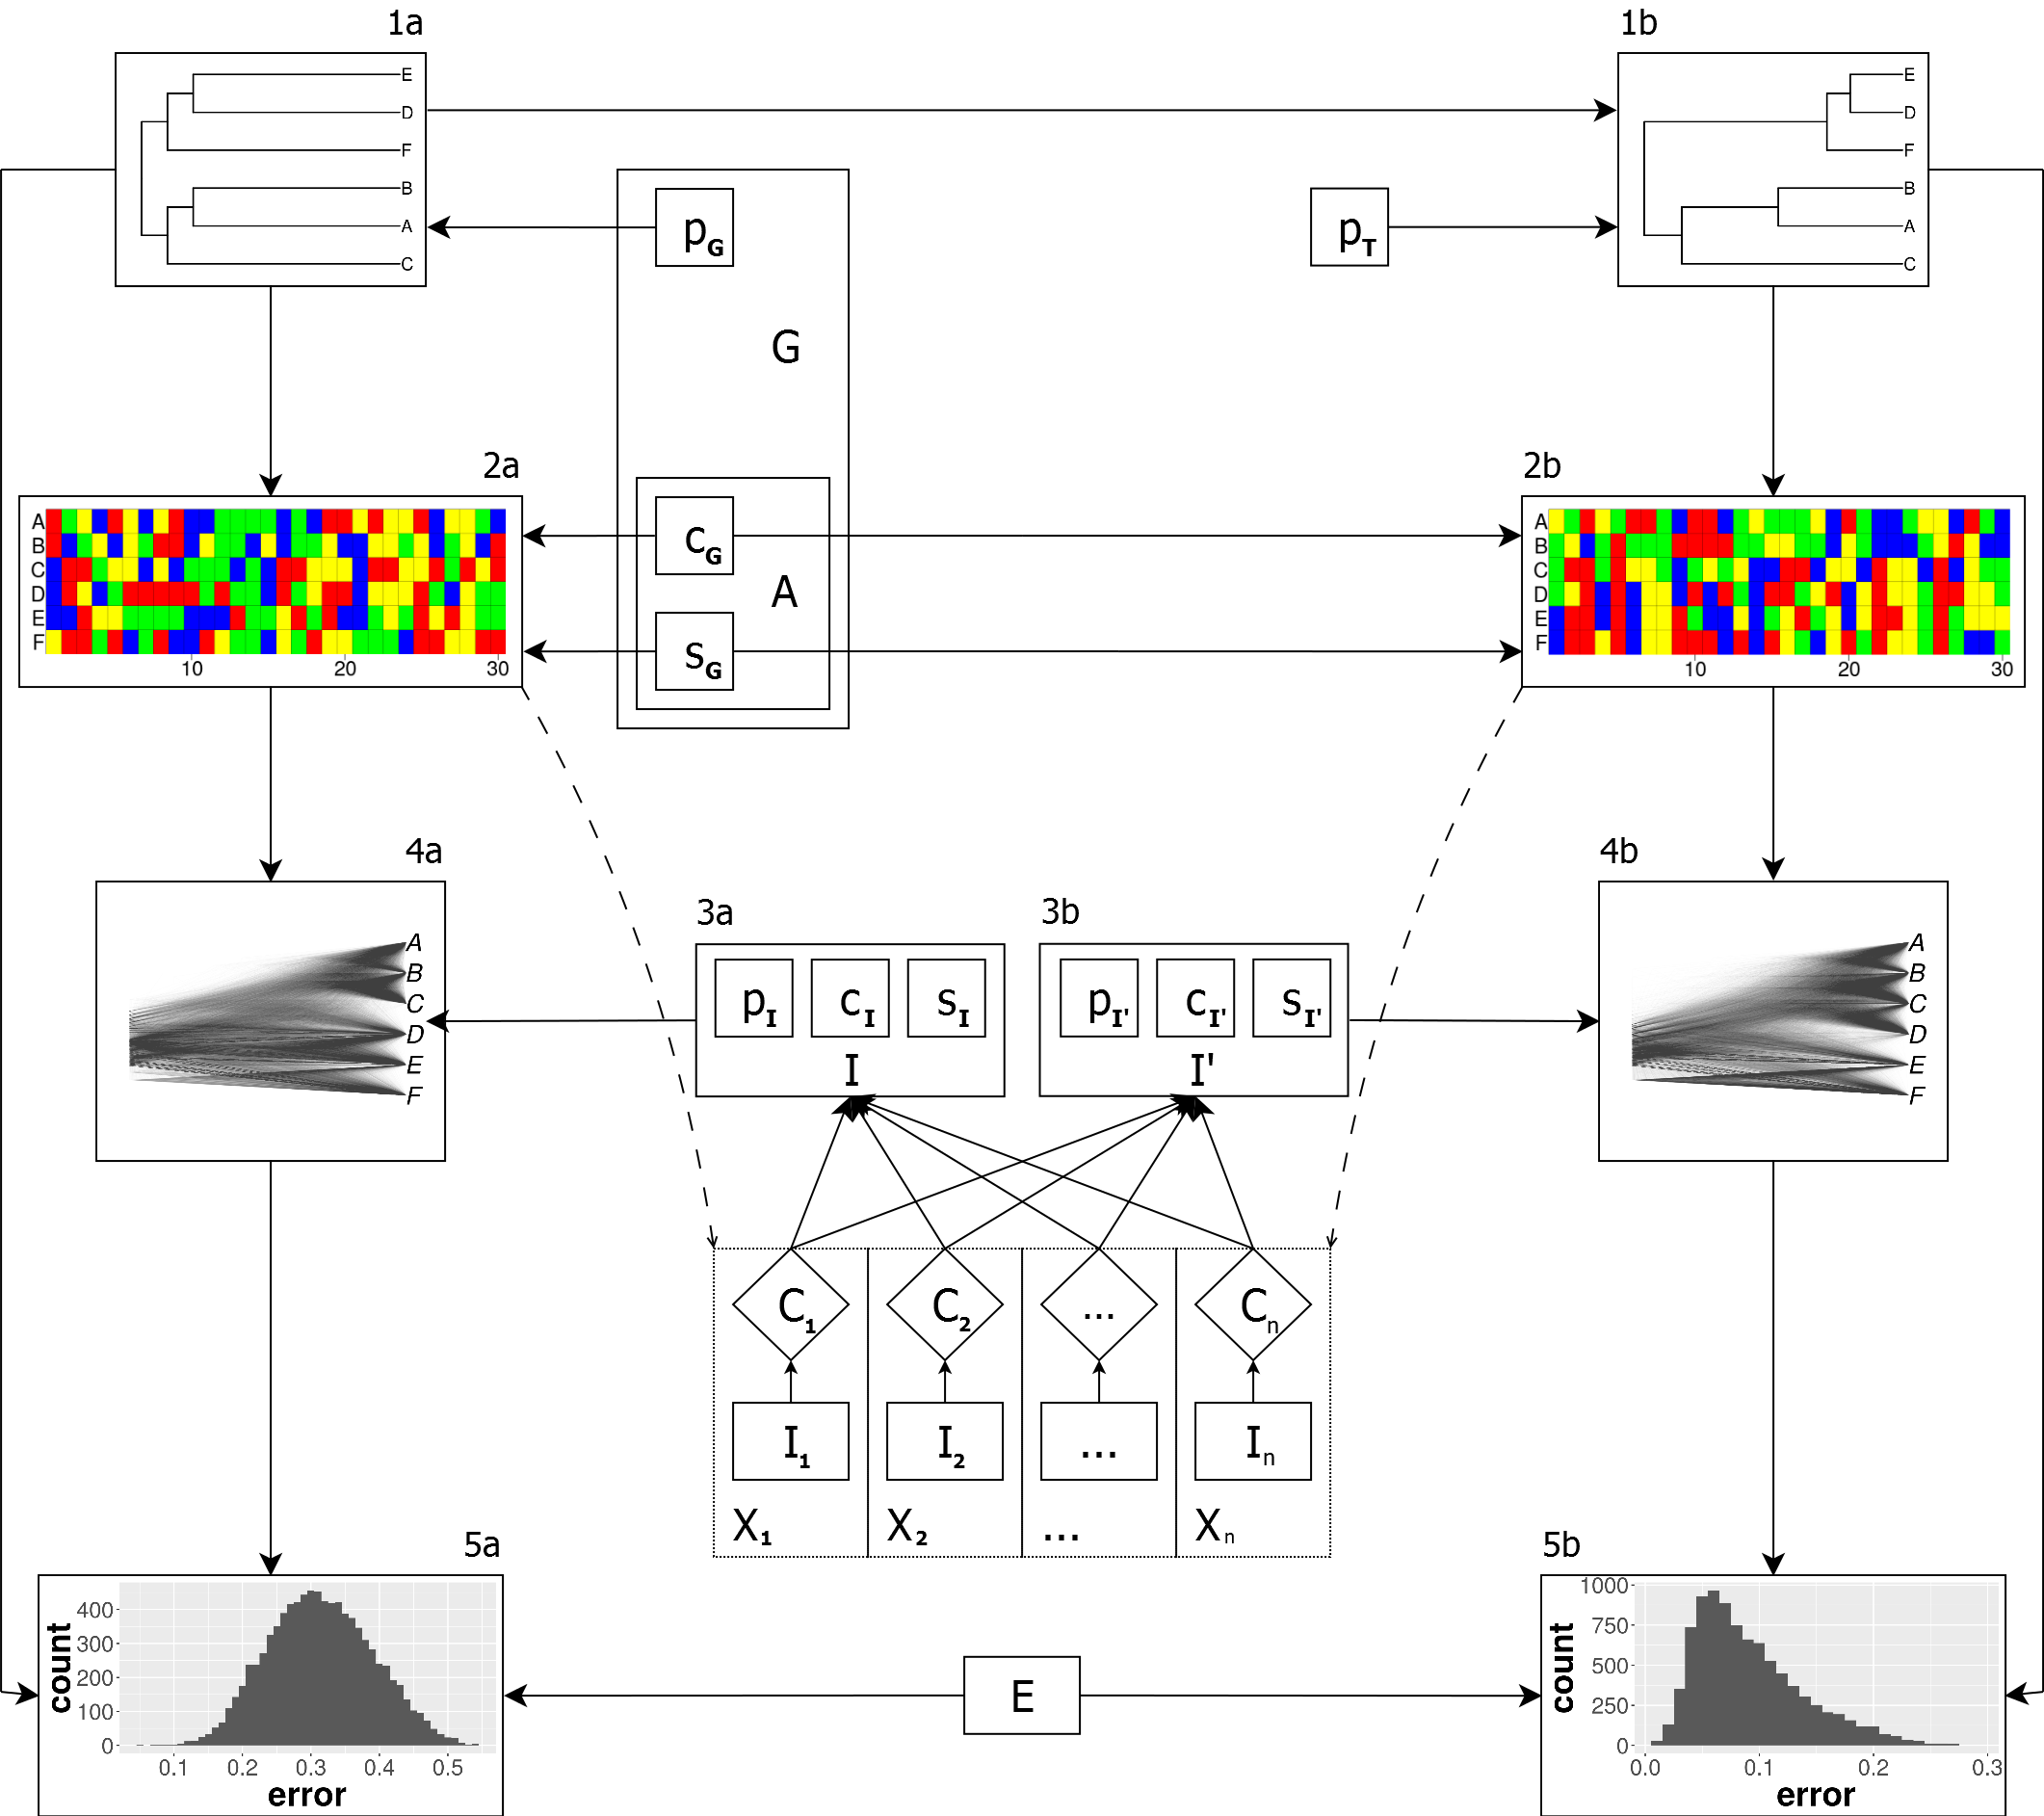
\includegraphics[width = 0.99\textwidth]{workflow4.png}
  \caption{
    \texttt{pirouette} pipeline.
    The pipeline starts from a phylogeny (1a) simulated by the 
    generative tree model 
    $\mathit{p_{G}}$.
    The phylogeny is converted to an alignment (2a) using the generative 
    alignment model 
    $\mathit{A} = (\mathit{c_{G}}, \mathit{s_{G}})$, composed of a clock model and a site model. 
    The user defines one or more experiments.
    For each candidate experiment $\mathit{X_{i}}$ 
    (a combination of inference model $\mathit{I_{i}}$ and condition $\mathit{C_{i}}$),
    if its condition $\mathit{C_{i}}$ is 
    satisfied (which can depend on the alignment), 
    the corresponding inference model $\mathit{I} = \mathit{I_{i}}$ is selected
    to be used in the next step.
    The inference models (3a) of the selected experiments use the alignment (2a) 
    to each create a Bayesian posterior of (parameter estimates and) 
    phylogenies (4a). 
    Each of the posteriors' trees is compared to the true phylogeny (1a) 
    using the error measure $\mathit{E}$, 
    resulting in an error distribution (5a). 
    Optionally, for each selected inference model a twin pipeline can be run.
    A twin phylogeny (1b) can be generated from the original 
    phylogeny (1a) using the twin tree model $\mathit{p_{t}}$, 
    selected among standard diversification models; 
    the default option is the standard BD model, 
    with parameters estimated from the original phylogeny.
    A twin alignment (2b) is then simulated from the twin phylogeny 
    using clock model $\mathit{c_{G}}$ and site model $\mathit{s_{G}}$ 
    imported from the generative model. 
    The twin pipeline follows the procedure of the main pipeline, 
    resulting in a twin error distribution (5b).
  }
  \label{fig:pipeline}
\end{figure}

The pipeline to assess the error BEAST2 makes in inferring this phylogeny 
contains the following steps:
\begin{enumerate}
  \item The user supplies one or (ideally) more phylogenies from a 
    new diversification model.
  \item From the given phylogeny an alignment is simulated 
    under a known alignment model $\mathit{A}$.
  \item From this alignment, according to the specified 
    inference conditions $\mathit{C}$, 
    an inference model $\mathit{I}$ is chosen (which may differ from the 
    generative model).
  \item The inference model and the alignment are used 
    to infer a posterior distribution of phylogenies.
  \item The phylogenies in the posterior are compared with the given phylogeny 
    to estimate the error made, according to 
    the error measure $\mathit{E}$ specified by the user.
\end{enumerate}

The pipeline is visualized in Fig.~\ref{fig:pipeline}. 
There is also the option to generate a 'twin tree', 
that goes through the same pipeline. 
The utility of this twin tree will be explained below.

The first step simulates an alignment from the given 
phylogeny (Fig.~\ref{fig:pipeline}, 1a $\rightarrow$ 2a).
For the sake of clarity, here we will assume the alignment consists
of DNA sequences, but one can also use other heritable material such as amino acids.
The user must specify a root sequence, a mutation rate and a site model.
\iffalse
The root sequence is the DNA sequence of the shared common ancestor of 
all species, and is set to four different equally-sized 
mononucleotide blocks by default, 
which helps interpreting the resulting alignment.
\fi
\new{ % 00008
The root sequence is the DNA sequence of the shared common ancestor of 
all species. By default it is set to four different equally-sized 
mononucleotide blocks (a block of length $n$ is a sequence in which the same character is repeated $n$ times), which helps interpreting the resulting alignment.
}
Supported nucleotide substitution models (part of a DNA
site model) are JC, HKY, TN and GTR (see Table \ref{tab:options} for
the meaning of these abbreviations).
JC is the default nucleotide substitution model (NSM),
in which the nucleotide substitution rates between all
nucleotides are equal and constant over time.

The second step (Fig.~\ref{fig:pipeline}, 3a)
selects one or more inference model(s) $I$ from 
a set of standard inference models $I_{1},\dots,I_{n}$.
For example, if the generative model is known and standard,
one can specify the inference model to be the same as the generative model.
If the tree model is unknown or non-standard - which is the primary motivation for this paper -, one can pick
a standard inference model which is considered to be closest to the true tree model.
Also, if we want to run only the inference
model that fits best to an alignment from a set of candidates,
one can specify these inference models as 
well (see section 'Candidate models').

The third step infers the posterior distributions,
using the simulated alignment (Fig.~\ref{fig:pipeline}, 2a $\rightarrow$ 4a),
and the inference models that were selected in the previous step (3a). 
For each selected experiment a posterior distribution is inferred, using the 
\verb;babette; [\cite{bilderbeek2018babette}] R package which makes use of BEAST2. 
This step usually takes up most of the pipeline's computation time.

The fourth step quantifies the inference error made. 
First the burn-in fraction is removed, i.e. the first phase of the 
Markov chain Monte Carlo (MCMC) run,
which samples an unrepresentative part of parameter and tree space. 
By default, \verb;pirouette; 
removes the first 10\% of the posterior.
From the remaining posterior, \verb;pirouette; 
creates an error distribution, by measuring the difference
between the true tree and each of the posterior 
trees (Fig.~\ref{fig:pipeline}, 4a $\rightarrow$ 5a).
The user can specify a function to quantify the differences between
the true and posterior trees. By default, the package uses the nLTT 
statistic [\cite{janzen2015approximate}], which is the absolute difference
between the normalized lineages-through-time plots of two trees.
The nLTT statistic is chosen, as it can operate on any two trees (regardless
of their crown ages and number of taxa) and its results have a clear range
from zero to one. This normalized result makes it possible to compare trees 
from a distribution of trees from any tree model.

\subsection{Twinning}\label{subsec:twinning}

Similar to lab experiments, \verb;pirouette; allows to perform
a control measurement, by use of a process we call twinning. 
In this context, this control results in an error distribution
that is the baseline error of the pipeline. The difference
between the 'true' and 'twin' error distributions is caused only
by the mismatch between the generative tree model and the assumed
tree prior.

The twinning process, $T$, encompasses two steps:
$T_1$, that generates a 'twin tree' (Fig.~\ref{fig:pipeline}, 1b) 
and $T_2$, which generates a 'twin alignment' (Fig.~\ref{fig:pipeline}, 2b).
Both twin tree and alignment will be analyzed in the same way 
as the true tree and alignment.

We define a phylogeny $\tau$ as the combination of
branching times $\Vec{t}$ and topology $\psi$, 
and denote as $\tau_{\mathit{G}}$ the phylogeny 
produced by a (possibly non-standard) generative diversification model, 
having branching times $\Vec{t}_{\mathit{G}}$ and 
topology $\psi_{\mathit{G}}$.

The first step ($T_1$) of the twinning process creates a tree $\tau_{\mathit{T}}$
with branching times $\Vec{t}_{\mathit{T}}$ while preserving the original
topology $\psi_{\mathit{G}}$:
\begin{align}
  \tau_{\mathit{G}} = (\Vec{t}_{\mathit{G}}, \psi_{\mathit{G}}) 
  \xrightarrow[]{\mathit{T_1}} 
  \tau_{\mathit{T}} = (\Vec{t}_{\mathit{T}}, \psi_{\mathit{G}})
\end{align}

\new{
  % 00007
  We choose to preserve the original topology to 
  increase the similarity between the twin to the original tree. 
  This works well in the cases of the birth-death or diversity-dependent models 
  we consider in our examples.
  However, this might not be suited for models in which branching times 
  are strongly influenced by topology.
}

\new{
  % 00003
  The default option for the twin diversification model $p_T$ 
  is to use the standard BD model.
}
\new{
  % 00009
  \verb;pirouette; has a built-in function to use a Yule model as well.
  Additionally, a user can specify a function to generate a twin tree
  from any speciation model, such as, for example, a coalescent model.
}

It is then possible to use the likelihood function 
$L_{\mathit{T}}$ for this diversification model to find 
the parameters $\theta^{*}_{\mathit{T}}$ 
(e.g. speciation and extinction rates, in case of a BD model) 
that maximize this likelihood applied 
to the true tree, conditioned on its number of tips $n_{\mathit{G}}$:
\begin{align}
    \max[L_{\mathit{T}}(\theta_{\mathit{T}}|\tau_{\mathit{G}}, n_{\mathit{G}})] 
\rightarrow \theta^{*}_{\mathit{T}}.
\end{align}
We use $\theta^{*}_{\mathit{T}}$ to simulate a number 
$n_{\mathit{T}} = n_{\mathit{G}}$ 
of branching times $\Vec{t}_{\mathit{T}}$ for the twin tree 
$\tau_{\mathit{T}}$, under the process $p_{T}$, 
while preserving the topology. 
We simulate the new branching times using the TESS 
package [\cite{TESS, hohna2016tess}].

The second step ($T_2$) of the twinning process simulates the twin alignment 
with the same clock model, site model and mutation rate 
used to simulate the original alignment. 
The twin alignment can be simulated in any user-defined way.
\verb;pirouette; supplies the option to have it simulated with
the same mutation rate as the true alignment. By default, however,
not only the same mutation rate is used, but also the total number of \new{substitution}s
matches the true alignment. The total number of \new{substitution}s is defined
as the amount of different nucleotides between the (known) root sequence
compared to the sequences at the tips.

\subsection{Candidate models}\label{subsec:candidates}

The user has to specify exactly one standard inference model,
but may be unsure which one to pick. To account for this, the user can
specify a set of candidate inference models. Each of these candidate inference models is run in an initial, relatively short, analysis; the candidate model with the highest 
evidence (i.e., marginal likelihood) will then be
used in another, longer, inference run, resulting in another error distribution.
The evidence for an inference model is estimated by nested 
sampling [\cite{russel2019model}], using the \verb;NS; BEAST2 package. 

If twinning is used, a candidate model that has the highest evidence for
the twin alignment is also used to create another error
distribution.

\subsection{Stochasticity caused by simulating phylogenies}

Finally, if the goal is to evaluate BEAST2's performance 
on a non-standard tree model, 
one must also consider the last source of stochasticity: 
the different phylogenies a tree model generates.
A single phylogeny cannot be considered as fully representative of the model. 
For this reason multiple phylogenies must be considered. 
If the number of considered phylogenies is high enough, 
the comparison between the main pipeline's aggregated error distribution 
and its twin counterpart leads to a fair evaluation 
of the new tree model with respect to the baseline error.

%%%%%%%%%%%%%%%%%%%%%%%%%%%%%%%%%%%%%%%%%%%%%%%%%%%%%%%%%%%%%%%%%%%%%%%%%%%%%%%%
\section{Usage}
%%%%%%%%%%%%%%%%%%%%%%%%%%%%%%%%%%%%%%%%%%%%%%%%%%%%%%%%%%%%%%%%%%%%%%%%%%%%%%%%

We show the usage of \verb;pirouette; on an tree generated 
by the non-standard diversity-dependent (DD) tree model [\citep{DDD, etienne2012diversity}],
which is a BD model with a speciation rate that is dependent on the number of species.

The code to reproduce our results can be found at  
\url{https://github.com/richelbilderbeek/pirouette_example_30}
and a simplified version is shown here for convenience:

\begin{lstlisting}[language=R]
library(pirouette)

# Create phylogeny
set.seed(314)
phylogeny <- create_exemplary_dd_tree(
  n_taxa = 6, 
  crown_age = 10,
  extinction_rate = 0.1
)

# Setup pirouette
pir_params <- create_std_pir_params(
  folder_name = "example_30"
)

# Do the runs
pir_out <- pir_run(
  phylogeny = phylogeny,
  pir_params = pir_params
)

# Save
library(ggplot2)
pir_plot(pir_out) +
  ggtitle("pirouette example 30") +
  ggsave("errors.png", width = 7, height = 7)

pir_save(
  phylogeny = phylogeny,
  pir_params = pir_params,
  pir_out = pir_out,
  folder_name = "example_30"
)
\end{lstlisting}

The DD tree that is generated by this code is as shown in Figure \ref{fig:dd_tree},
which has an arbitrarily chosen crown age of 10 time units and 6 tips for an extinction rate of 0.1. The carrying-capacity is also set at 6. The initial speciation rate $\lambda_0$ is chosen such that the expected number of species in a constant-rate BD model would be equal to the number of tips, which amounts to $\lambda_0 = 0.63$.

\begin{figure}[H]
  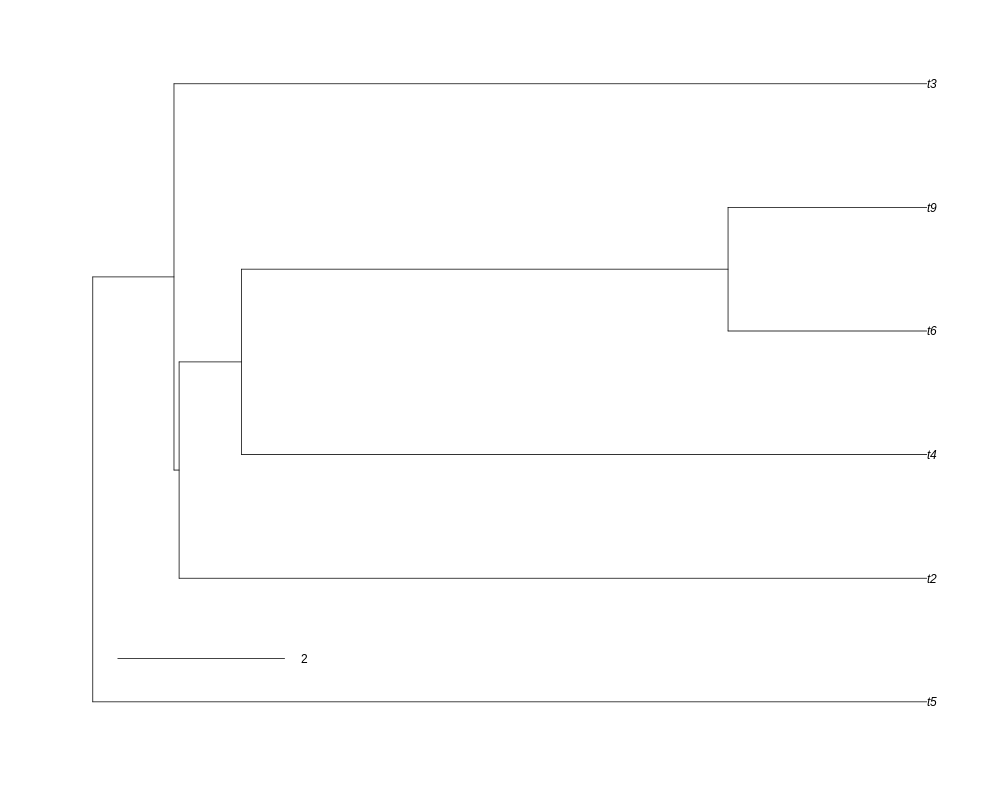
\includegraphics[width=\textwidth]{pirouette_example_30/example_30_314/true_tree.png}
  \caption{
    The example tree resulting from a diversity-dependent (DD) simulation.
  }
  \label{fig:dd_tree}
\end{figure}

Using the default \verb;pirouette; settings,
the error distribution shown in Figure \ref{fig:example_30}
is produced.

\begin{figure}[H]
  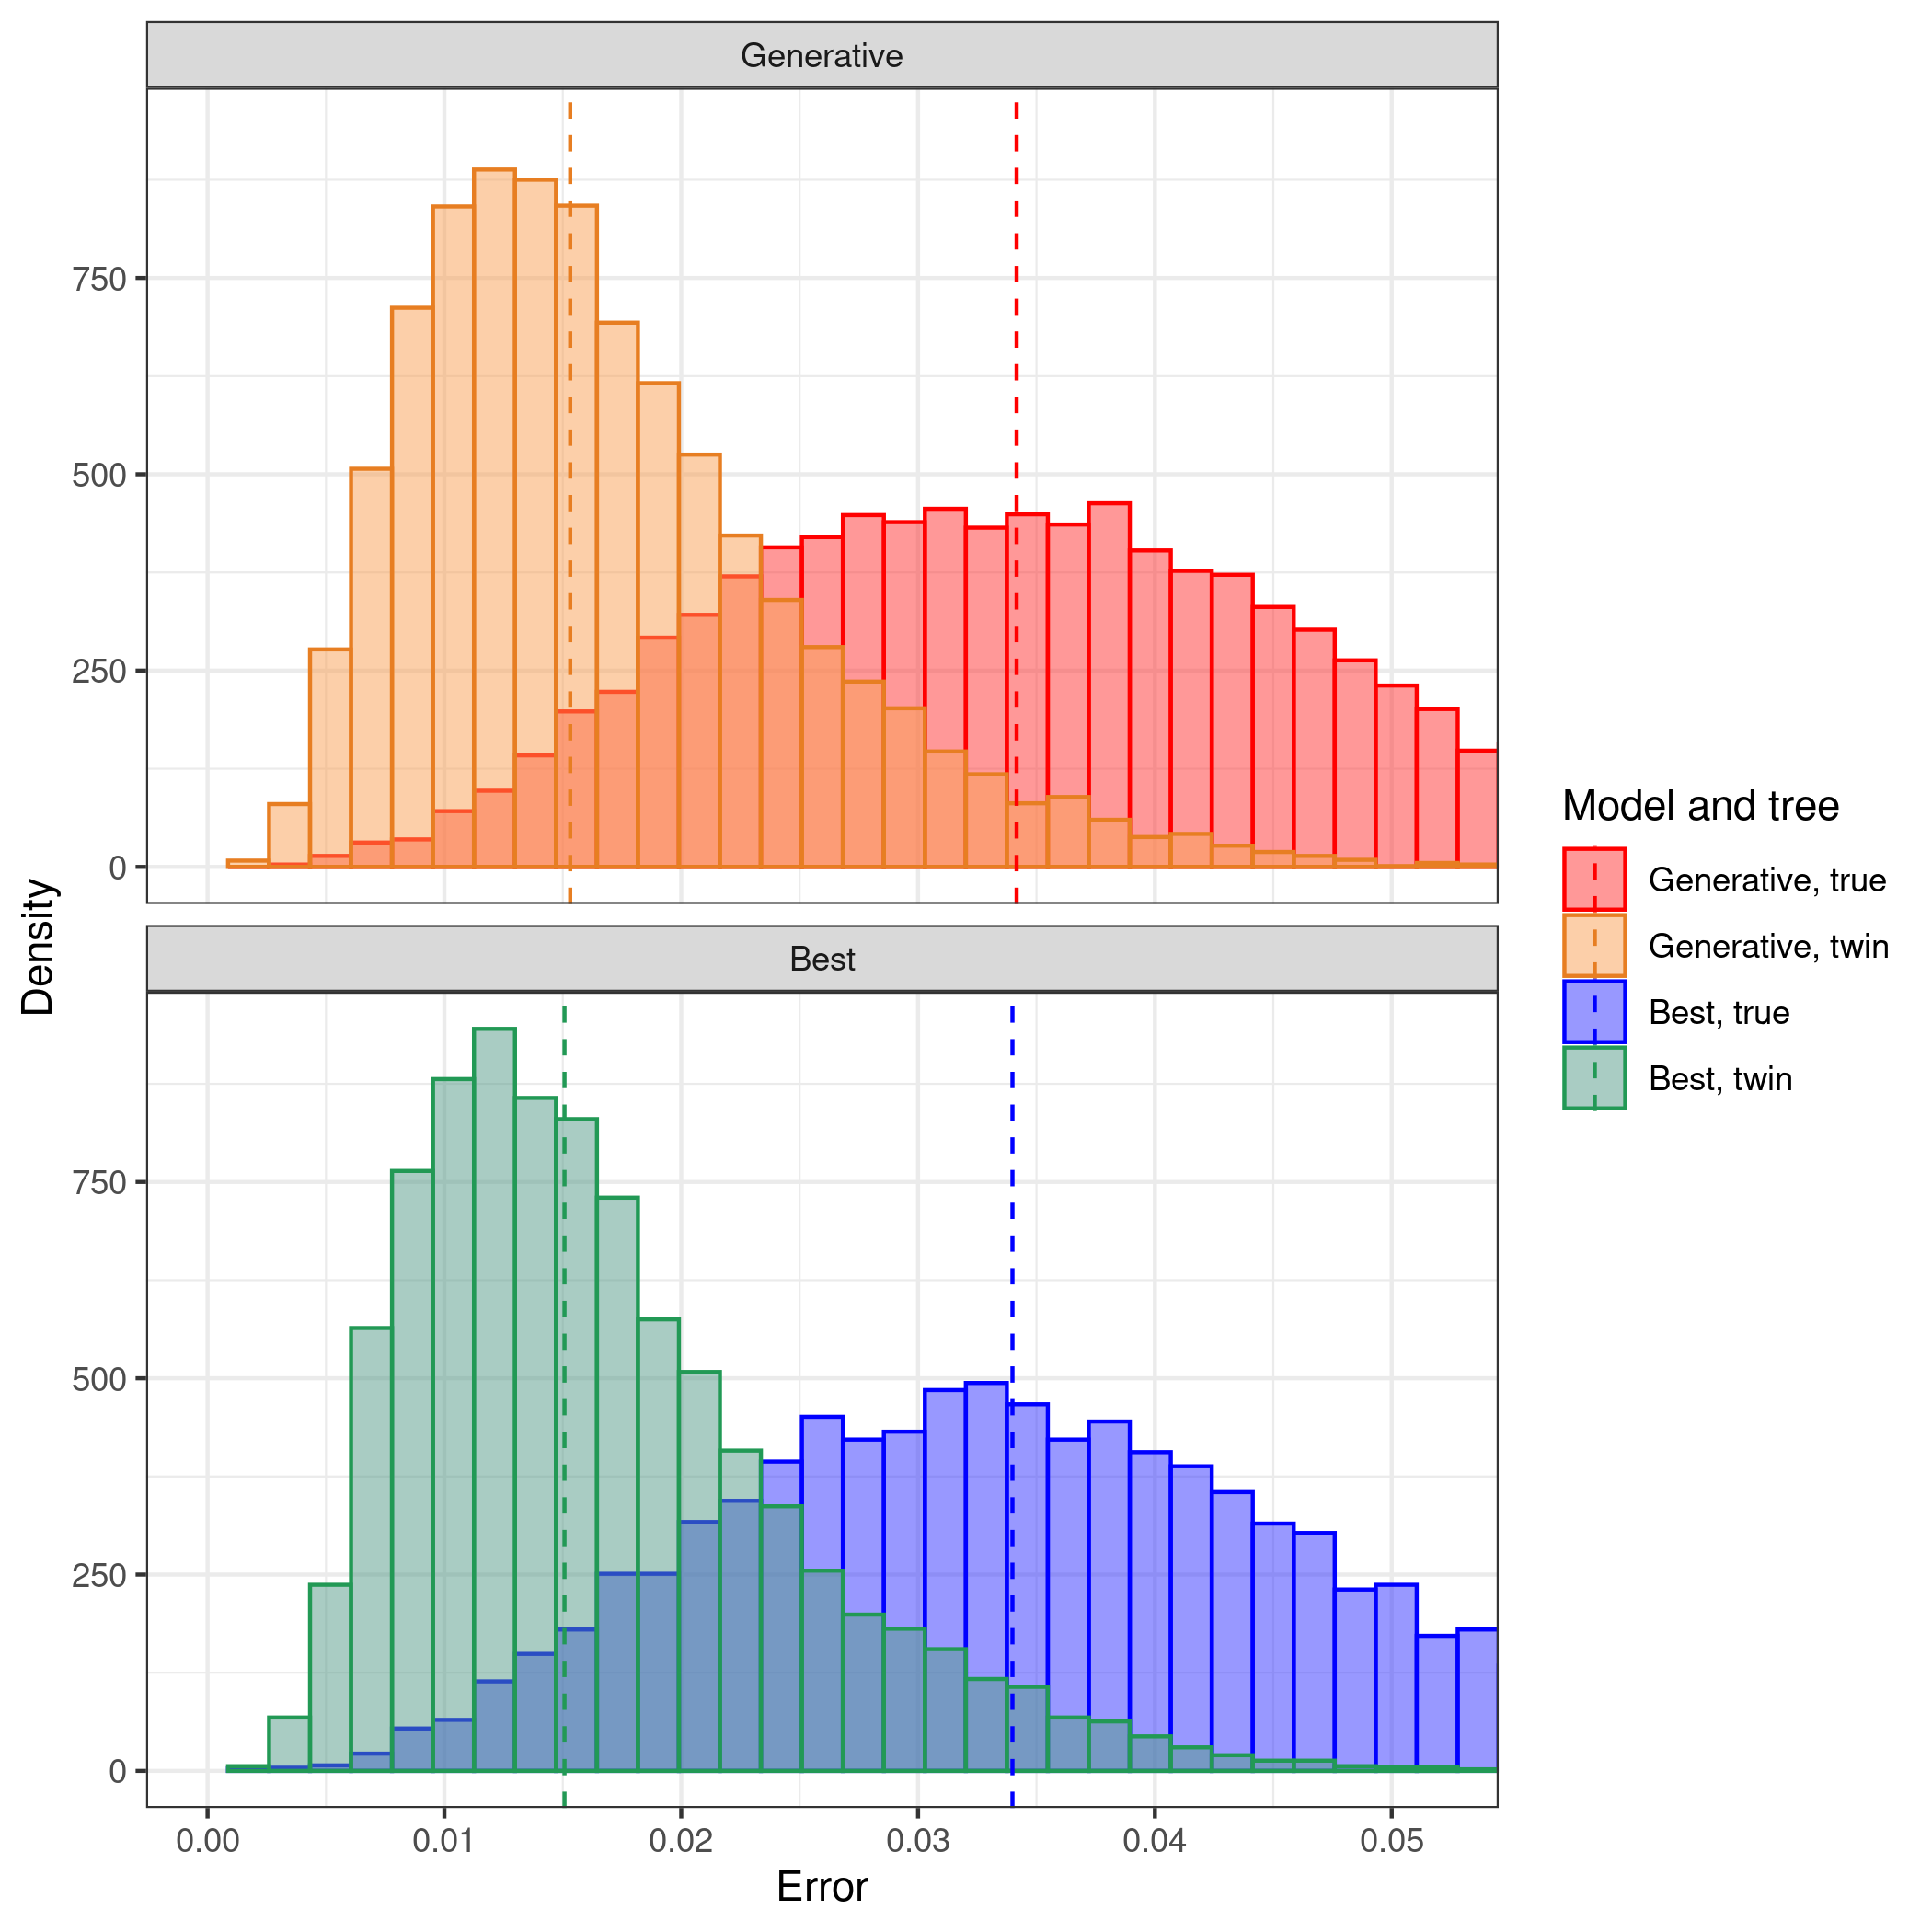
\includegraphics[width=\textwidth]{pirouette_example_30/errors.png}
  \caption{
    The inference error made 
    for an assumed generative tree model and best candidate model,
    compared with the error obtained for the twin tree.
    The assumed generative tree model is the model assumed to be closest to
    the actual generative tree model that generated the true tree.
    The twin distributions show the baseline inference error.
    Vertical dashed lines show the median error value per distribution.
  }
  \label{fig:example_30}
\end{figure}

In the upper panel of Figure \ref{fig:example_30},
we can see that the error distributions of the assumed generative model
differ strongly between the true and twin tree. 
This difference shows the extent of the mismatch between
the actual tree model (which is DD) and the (BD) tree prior used.
Because these distributions are distinctively different,
the inference error we make when using an 
incorrect (that is, BD) tree prior on a DD tree
is profound.

Comparing the upper and lower panel of Figure \ref{fig:example_30}, 
we can see that the best
candidate model is only slightly better at inferring the true tree,
than the assumed generative model, thereby showing that they cannot compensate for the true generative tree model not being among the inference models.

The candidate model that had highest evidence given the simulated alignment,
was JC, RLN, BD (see Table \ref{tab:options} for the meaning of these 
abbreviations). JC was indeed the site model used when simulating the
alignments. The RLN clock model is an unexpected choice: the RLN clock
model assumes that mutation rates differ between lineages, whereas the
alignment was simulated with equal mutation rates for all lineages.
The BD model is indeed closer to the DD model than Yule, as both BD and DD
model allow for extinction, while Yule does not.

%%%%%%%%%%%%%%%%%%%%%%%%%%%%%%%%%%%%%%%%%%%%%%%%%%%%%%%%%%%%%%%%%%%%%%%%%%%%%%%%
\section{Discussion}
%%%%%%%%%%%%%%%%%%%%%%%%%%%%%%%%%%%%%%%%%%%%%%%%%%%%%%%%%%%%%%%%%%%%%%%%%%%%%%%%

We showed how to use \verb;pirouette; to quantify the \new{impact} of a 
tree prior in Bayesian phylogenetics, assuming the simplest standard 
tree model possible.
In principle any other standard tree model can be assumed, 
but we chose to provide the simplest example.

Figure~\ref{fig:example_30} illustrates the primary result of our pipeline: 
it shows the error distributions for the true tree and the twin tree 
when either the (assumed) generating model or the best candidate model is used in inference. 
The clear difference between the error distributions 
for the true tree and the twin tree suggests 
that the choice of tree prior does matter.
We note, however, that only one tree from a novel tree model
is not enough to determine the \new{impact} of using an incorrect
tree prior. Instead, a distribution 
of multiple trees, generated by the novel tree model, should be used. In the supplementary material we have provided some examples.

Like most phylogenetic experiments, the setup of \verb;pirouette;
involves many choices. A prime example is the
length of the simulated DNA sequence. One expects that the inference error
decreases for longer DNA sequences. We investigated this
superficially and confirmed this prediction (see the supplementary materials). 
However, we note that for longer DNA sequences, the assumption 
of constant substitution rates may become less realistic 
and hence longer sequences may require more parameters. 
Hence, simply getting longer sequences will not always lead to a drastic 
reduction of the influence of the species tree prior.
Fortunately, \verb;pirouette; provides a pipeline that works for all choices.

Interpreting the results of \verb;pirouette; is up to the user; 
\verb;pirouette; does not answer the question 
whether the inference error is too large to trust the inferred tree. The user is encouraged to use different statistics to measure the error. The nLTT statistic is
a promising starting point, as it can compare any two trees and 
results in an error distribution of known range, but one may also explore other statistics.
In principle, \verb;pirouette; allows for this, but in our example we used a diversification model (DD) that only deviates from the Yule and BD models in the temporal branching pattern, not in the topology.
\new{
    % 00007
    For models that make different predictions on topology, the twinning process should be modified in line with it.
}

As noted in the introduction, Duch\^{e}ne and colleagues [\cite{duchene2018phylodynamic}],
also developed a method to assess the adequacy of a tree model
on empirical trees. They simulate trees from the posterior distribution of the parameters and then compare this to the originally inferred tree using tree statistics, to determine whether the assumed tree model in inference indeed generates the tree as inferred. This is useful if these trees match, but when they do not, this does not mean that the inferred tree is incorrect; if sufficient data is available the species tree prior may not be important, and hence the inference may be adequate even though the assumed species tree prior is not. In short, the approach is applied to empirical trees and compares the posterior and prior distribution of trees (with the latter generated with the posterior parameters!).
\verb;pirouette; aims to identify when assuming standard priors for the species tree leads to incorrect inference if one believes more complex diversification models are operating than can be currently accommodated in inference. In short, our approach applies to simulated trees and compares the posterior distributions of trees generated with a standard and non-standard model, but inferred with a standard one. The two methods therefore complement one another.

However, we note that the \verb;pirouette; pipeline is not restricted 
to exploring the effects of a new species tree model. 
The pipeline can also be used to explore the effects of non-standard 
clock or site models, such as relaxed clock models with a non-standard 
distribution, correlated substitutions on sister lineages, or elevated 
substitutions rates during speciation events. 
It is, however, beyond the scope of this paper to discuss all these options 
in more detail.

In conclusion, \verb;pirouette; can show the errors to be expected
when the model assumed in inference is different from the 
actual generative model.
The user can then judge whether or not this new model should be implemented in our Bayesian phylogenetic tool. 

%%%%%%%%%%%%%%%%%%%%%%%%%%%%%%%%%%%%%%%%%%%%%%%%%%%%%%%%%%%%%%%%%%%%%%%%%%%%%%%%
\section{Acknowledgments}
%%%%%%%%%%%%%%%%%%%%%%%%%%%%%%%%%%%%%%%%%%%%%%%%%%%%%%%%%%%%%%%%%%%%%%%%%%%%%%%%

We thank the Center for Information Technology of the University 
of Groningen for its support and for providing access to the Peregrine 
high performance computing cluster. 
We thank the Netherlands 
Organization for Scientific Research (NWO) for financial support 
through a VICI grant awarded to RSE.

%%%%%%%%%%%%%%%%%%%%%%%%%%%%%%%%%%%%%%%%%%%%%%%%%%%%%%%%%%%%%%%%%%%%%%%%%%%%%%%%
\section{Data Accessibility}
%%%%%%%%%%%%%%%%%%%%%%%%%%%%%%%%%%%%%%%%%%%%%%%%%%%%%%%%%%%%%%%%%%%%%%%%%%%%%%%%

All code is archived at 
\url{http://github.com/richelbilderbeek/pirouette_article},
with DOI \url{https://doi.org/12.3456/zenodo.1234567}.

%%%%%%%%%%%%%%%%%%%%%%%%%%%%%%%%%%%%%%%%%%%%%%%%%%%%%%%%%%%%%%%%%%%%%%%%%%%%%%%%
\section{Author contributions}
%%%%%%%%%%%%%%%%%%%%%%%%%%%%%%%%%%%%%%%%%%%%%%%%%%%%%%%%%%%%%%%%%%%%%%%%%%%%%%%%

RJCB, GL and RSE conceived the idea for the package. 
RJCB created, tested and revised the package.
GL provided major contributions to the package.
RJCB wrote the first draft of the manuscript, 
GL and RSE contributed to revisions.

%%%%%%%%%%%%%%%%%%%%%%%%%%%%%%%%%%%%%%%%%%%%%%%%%%%%%%%%%%%%%%%%%%%%%%%%%%%%%%%%
% Bibliography
%%%%%%%%%%%%%%%%%%%%%%%%%%%%%%%%%%%%%%%%%%%%%%%%%%%%%%%%%%%%%%%%%%%%%%%%%%%%%%%%
% MEE style
\bibliographystyle{pirouette_mee}
\bibliography{pirouette_article}
%%%%%%%%%%%%%%%%%%%%%%%%%%%%%%%%%%%%%%%%%%%%%%%%%%%%%%%%%%%%%%%%%%%%%%%%%%%%%%%%

